\chapter{}

\begin{figure}[htp]
    \centering
    \includegraphics[width=1\textwidth]{imagenes/fitness_charts/results/real/waveform5000/optimizer_boxplot_fitness_knn_r.png}
    \caption{\textit{Boxplot} waveform5000 - knn - real}

\end{figure}

\begin{figure}[htp]
    \centering
    \includegraphics[width=1\textwidth]{imagenes/fitness_charts/results/real/yeast/optimizer_boxplot_fitness_knn_r.png}
    \caption{\textit{Boxplot} yeast - knn - real}

\end{figure}

\begin{figure}[htp]
    \centering
    \includegraphics[width=1\textwidth]{imagenes/fitness_charts/results/real/spectf-heart/optimizer_boxplot_fitness_knn_r.png}
    \caption{\textit{Boxplot} spectf-heart - knn - real}

\end{figure}

\begin{figure}[htp]
    \centering
    \includegraphics[width=1\textwidth]{imagenes/fitness_charts/results/real/dermatology/optimizer_boxplot_fitness_knn_r.png}
    \caption{\textit{Boxplot} dermatology - knn - real}

\end{figure}

\begin{figure}[htp]
    \centering
    \includegraphics[width=1\textwidth]{imagenes/fitness_charts/results/real/wdbc/optimizer_boxplot_fitness_knn_r.png}
    \caption{\textit{Boxplot} wdbc - knn - real}

\end{figure}

\begin{figure}[htp]
    \centering
    \includegraphics[width=1\textwidth]{imagenes/fitness_charts/results/real/breast-cancer/optimizer_boxplot_fitness_knn_r.png}
    \caption{\textit{Boxplot} breast-cancer - knn - real}

\end{figure}

\begin{figure}[htp]
    \centering
    \includegraphics[width=1\textwidth]{imagenes/fitness_charts/results/real/wine/optimizer_boxplot_fitness_knn_r.png}
    \caption{\textit{Boxplot} wine - knn - real}

\end{figure}

\begin{figure}[htp]
    \centering
    \includegraphics[width=1\textwidth]{imagenes/fitness_charts/results/real/spambase-460/optimizer_boxplot_fitness_knn_r.png}
    \caption{\textit{Boxplot} spambase-460 - knn - real}

\end{figure}

\begin{figure}[htp]
    \centering
    \includegraphics[width=1\textwidth]{imagenes/fitness_charts/results/real/parkinsons/optimizer_boxplot_fitness_knn_r.png}
    \caption{\textit{Boxplot} parkinsons - knn - real}

\end{figure}

\begin{figure}[htp]
    \centering
    \includegraphics[width=1\textwidth]{imagenes/fitness_charts/results/real/sonar/optimizer_boxplot_fitness_knn_r.png}
    \caption{\textit{Boxplot} sonar - knn - real}

\end{figure}

\begin{figure}[htp]
    \centering
    \includegraphics[width=1\textwidth]{imagenes/fitness_charts/results/real/zoo/optimizer_boxplot_fitness_knn_r.png}
    \caption{\textit{Boxplot} zoo - knn - real}

\end{figure}

\begin{figure}[htp]
    \centering
    \includegraphics[width=1\textwidth]{imagenes/fitness_charts/results/real/diabetes/optimizer_boxplot_fitness_knn_r.png}
    \caption{\textit{Boxplot} diabetes - knn - real}

\end{figure}

\begin{figure}[htp]
    \centering
    \includegraphics[width=1\textwidth]{imagenes/fitness_charts/results/real/iris/optimizer_boxplot_fitness_knn_r.png}
    \caption{\textit{Boxplot} iris - knn - real}

\end{figure}

\begin{figure}[htp]
    \centering
    \includegraphics[width=1\textwidth]{imagenes/fitness_charts/results/real/ecoli/optimizer_boxplot_fitness_knn_r.png}
    \caption{\textit{Boxplot} ecoli - knn - real}

\end{figure}

\begin{figure}[htp]
    \centering
    \includegraphics[width=1\textwidth]{imagenes/fitness_charts/results/real/waveform5000/optimizer_boxplot_fitness_svc_r.png}
    \caption{\textit{Boxplot} waveform5000 - svc - real}

\end{figure}

\begin{figure}[htp]
    \centering
    \includegraphics[width=1\textwidth]{imagenes/fitness_charts/results/real/yeast/optimizer_boxplot_fitness_svc_r.png}
    \caption{\textit{Boxplot} yeast - svc - real}

\end{figure}

\begin{figure}[htp]
    \centering
    \includegraphics[width=1\textwidth]{imagenes/fitness_charts/results/real/spectf-heart/optimizer_boxplot_fitness_svc_r.png}
    \caption{\textit{Boxplot} spectf-heart - svc - real}

\end{figure}

\begin{figure}[htp]
    \centering
    \includegraphics[width=1\textwidth]{imagenes/fitness_charts/results/real/dermatology/optimizer_boxplot_fitness_svc_r.png}
    \caption{\textit{Boxplot} dermatology - svc - real}

\end{figure}

\begin{figure}[htp]
    \centering
    \includegraphics[width=1\textwidth]{imagenes/fitness_charts/results/real/wdbc/optimizer_boxplot_fitness_svc_r.png}
    \caption{\textit{Boxplot} wdbc - svc - real}

\end{figure}

\begin{figure}[htp]
    \centering
    \includegraphics[width=1\textwidth]{imagenes/fitness_charts/results/real/breast-cancer/optimizer_boxplot_fitness_svc_r.png}
    \caption{\textit{Boxplot} breast-cancer - svc - real}

\end{figure}

\begin{figure}[htp]
    \centering
    \includegraphics[width=1\textwidth]{imagenes/fitness_charts/results/real/wine/optimizer_boxplot_fitness_svc_r.png}
    \caption{\textit{Boxplot} wine - svc - real}

\end{figure}

\begin{figure}[htp]
    \centering
    \includegraphics[width=1\textwidth]{imagenes/fitness_charts/results/real/spambase-460/optimizer_boxplot_fitness_svc_r.png}
    \caption{\textit{Boxplot} spambase-460 - svc - real}

\end{figure}

\begin{figure}[htp]
    \centering
    \includegraphics[width=1\textwidth]{imagenes/fitness_charts/results/real/parkinsons/optimizer_boxplot_fitness_svc_r.png}
    \caption{\textit{Boxplot} parkinsons - svc - real}

\end{figure}

\begin{figure}[htp]
    \centering
    \includegraphics[width=1\textwidth]{imagenes/fitness_charts/results/real/sonar/optimizer_boxplot_fitness_svc_r.png}
    \caption{\textit{Boxplot} sonar - svc - real}

\end{figure}

\begin{figure}[htp]
    \centering
    \includegraphics[width=1\textwidth]{imagenes/fitness_charts/results/real/zoo/optimizer_boxplot_fitness_svc_r.png}
    \caption{\textit{Boxplot} zoo - svc - real}

\end{figure}

\begin{figure}[htp]
    \centering
    \includegraphics[width=1\textwidth]{imagenes/fitness_charts/results/real/diabetes/optimizer_boxplot_fitness_svc_r.png}
    \caption{\textit{Boxplot} diabetes - svc - real}

\end{figure}

\begin{figure}[htp]
    \centering
    \includegraphics[width=1\textwidth]{imagenes/fitness_charts/results/real/iris/optimizer_boxplot_fitness_svc_r.png}
    \caption{\textit{Boxplot} iris - svc - real}

\end{figure}

\begin{figure}[htp]
    \centering
    \includegraphics[width=1\textwidth]{imagenes/fitness_charts/results/real/ecoli/optimizer_boxplot_fitness_svc_r.png}
    \caption{\textit{Boxplot} ecoli - svc - real}

\end{figure}

\begin{figure}[htp]
    \centering
    \includegraphics[width=1\textwidth]{imagenes/fitness_charts/results/binary/waveform5000/optimizer_boxplot_fitness_knn_b.png}
    \caption{\textit{Boxplot} waveform5000 - knn - binary}

\end{figure}

\begin{figure}[htp]
    \centering
    \includegraphics[width=1\textwidth]{imagenes/fitness_charts/results/binary/yeast/optimizer_boxplot_fitness_knn_b.png}
    \caption{\textit{Boxplot} yeast - knn - binary}

\end{figure}

\begin{figure}[htp]
    \centering
    \includegraphics[width=1\textwidth]{imagenes/fitness_charts/results/binary/spectf-heart/optimizer_boxplot_fitness_knn_b.png}
    \caption{\textit{Boxplot} spectf-heart - knn - binary}

\end{figure}

\begin{figure}[htp]
    \centering
    \includegraphics[width=1\textwidth]{imagenes/fitness_charts/results/binary/dermatology/optimizer_boxplot_fitness_knn_b.png}
    \caption{\textit{Boxplot} dermatology - knn - binary}

\end{figure}

\begin{figure}[htp]
    \centering
    \includegraphics[width=1\textwidth]{imagenes/fitness_charts/results/binary/wdbc/optimizer_boxplot_fitness_knn_b.png}
    \caption{\textit{Boxplot} wdbc - knn - binary}

\end{figure}

\begin{figure}[htp]
    \centering
    \includegraphics[width=1\textwidth]{imagenes/fitness_charts/results/binary/breast-cancer/optimizer_boxplot_fitness_knn_b.png}
    \caption{\textit{Boxplot} breast-cancer - knn - binary}

\end{figure}

\begin{figure}[htp]
    \centering
    \includegraphics[width=1\textwidth]{imagenes/fitness_charts/results/binary/wine/optimizer_boxplot_fitness_knn_b.png}
    \caption{\textit{Boxplot} wine - knn - binary}

\end{figure}

\begin{figure}[htp]
    \centering
    \includegraphics[width=1\textwidth]{imagenes/fitness_charts/results/binary/spambase-460/optimizer_boxplot_fitness_knn_b.png}
    \caption{\textit{Boxplot} spambase-460 - knn - binary}

\end{figure}

\begin{figure}[htp]
    \centering
    \includegraphics[width=1\textwidth]{imagenes/fitness_charts/results/binary/parkinsons/optimizer_boxplot_fitness_knn_b.png}
    \caption{\textit{Boxplot} parkinsons - knn - binary}

\end{figure}

\begin{figure}[htp]
    \centering
    \includegraphics[width=1\textwidth]{imagenes/fitness_charts/results/binary/sonar/optimizer_boxplot_fitness_knn_b.png}
    \caption{\textit{Boxplot} sonar - knn - binary}

\end{figure}

\begin{figure}[htp]
    \centering
    \includegraphics[width=1\textwidth]{imagenes/fitness_charts/results/binary/zoo/optimizer_boxplot_fitness_knn_b.png}
    \caption{\textit{Boxplot} zoo - knn - binary}

\end{figure}

\begin{figure}[htp]
    \centering
    \includegraphics[width=1\textwidth]{imagenes/fitness_charts/results/binary/diabetes/optimizer_boxplot_fitness_knn_b.png}
    \caption{\textit{Boxplot} diabetes - knn - binary}

\end{figure}

\begin{figure}[htp]
    \centering
    \includegraphics[width=1\textwidth]{imagenes/fitness_charts/results/binary/iris/optimizer_boxplot_fitness_knn_b.png}
    \caption{\textit{Boxplot} iris - knn - binary}

\end{figure}

\begin{figure}[htp]
    \centering
    \includegraphics[width=1\textwidth]{imagenes/fitness_charts/results/binary/ecoli/optimizer_boxplot_fitness_knn_b.png}
    \caption{\textit{Boxplot} ecoli - knn - binary}

\end{figure}

\begin{figure}[htp]
    \centering
    \includegraphics[width=1\textwidth]{imagenes/fitness_charts/results/binary/waveform5000/optimizer_boxplot_fitness_svc_b.png}
    \caption{\textit{Boxplot} waveform5000 - svc - binary}

\end{figure}

\begin{figure}[htp]
    \centering
    \includegraphics[width=1\textwidth]{imagenes/fitness_charts/results/binary/yeast/optimizer_boxplot_fitness_svc_b.png}
    \caption{\textit{Boxplot} yeast - svc - binary}

\end{figure}

\begin{figure}[htp]
    \centering
    \includegraphics[width=1\textwidth]{imagenes/fitness_charts/results/binary/spectf-heart/optimizer_boxplot_fitness_svc_b.png}
    \caption{\textit{Boxplot} spectf-heart - svc - binary}

\end{figure}

\begin{figure}[htp]
    \centering
    \includegraphics[width=1\textwidth]{imagenes/fitness_charts/results/binary/dermatology/optimizer_boxplot_fitness_svc_b.png}
    \caption{\textit{Boxplot} dermatology - svc - binary}

\end{figure}

\begin{figure}[htp]
    \centering
    \includegraphics[width=1\textwidth]{imagenes/fitness_charts/results/binary/wdbc/optimizer_boxplot_fitness_svc_b.png}
    \caption{\textit{Boxplot} wdbc - svc - binary}

\end{figure}

\begin{figure}[htp]
    \centering
    \includegraphics[width=1\textwidth]{imagenes/fitness_charts/results/binary/breast-cancer/optimizer_boxplot_fitness_svc_b.png}
    \caption{\textit{Boxplot} breast-cancer - svc - binary}

\end{figure}

\begin{figure}[htp]
    \centering
    \includegraphics[width=1\textwidth]{imagenes/fitness_charts/results/binary/wine/optimizer_boxplot_fitness_svc_b.png}
    \caption{\textit{Boxplot} wine - svc - binary}

\end{figure}

\begin{figure}[htp]
    \centering
    \includegraphics[width=1\textwidth]{imagenes/fitness_charts/results/binary/spambase-460/optimizer_boxplot_fitness_svc_b.png}
    \caption{\textit{Boxplot} spambase-460 - svc - binary}

\end{figure}

\begin{figure}[htp]
    \centering
    \includegraphics[width=1\textwidth]{imagenes/fitness_charts/results/binary/parkinsons/optimizer_boxplot_fitness_svc_b.png}
    \caption{\textit{Boxplot} parkinsons - svc - binary}

\end{figure}

\begin{figure}[htp]
    \centering
    \includegraphics[width=1\textwidth]{imagenes/fitness_charts/results/binary/sonar/optimizer_boxplot_fitness_svc_b.png}
    \caption{\textit{Boxplot} sonar - svc - binary}

\end{figure}

\begin{figure}[htp]
    \centering
    \includegraphics[width=1\textwidth]{imagenes/fitness_charts/results/binary/zoo/optimizer_boxplot_fitness_svc_b.png}
    \caption{\textit{Boxplot} zoo - svc - binary}

\end{figure}

\begin{figure}[htp]
    \centering
    \includegraphics[width=1\textwidth]{imagenes/fitness_charts/results/binary/diabetes/optimizer_boxplot_fitness_svc_b.png}
    \caption{\textit{Boxplot} diabetes - svc - binary}

\end{figure}

\begin{figure}[htp]
    \centering
    \includegraphics[width=1\textwidth]{imagenes/fitness_charts/results/binary/iris/optimizer_boxplot_fitness_svc_b.png}
    \caption{\textit{Boxplot} iris - svc - binary}

\end{figure}

\begin{figure}[htp]
    \centering
    \includegraphics[width=1\textwidth]{imagenes/fitness_charts/results/binary/ecoli/optimizer_boxplot_fitness_svc_b.png}
    \caption{\textit{Boxplot} ecoli - svc - binary}

\end{figure}

\begin{sidewaystable}[htp]
    \centering
    \begin{adjustbox}{width=\linewidth}
        \begin{tabular}{llllllllllllll}
            \toprule
            {}    & abco      & aco       & ba        & cs            & da        & de        & dummy         & fa        & ga        & goa       & gwo           & pso           & woa       \\
            \midrule
            abco  & -         & + (0.083) & + (0.008) & + (0.012)     & + (0.151) & + (0.020) & - (0.018)     & + (0.105) & + (0.012) & + (0.252) & + (0.003)     & + (0.001)     & + (0.012) \\
            aco   & - (0.083) & -         & = (0.514) & = (0.561)     & = (0.679) & = (0.934) & - (0.012)     & + (0.443) & = (0.754) & - (0.389) & + (0.055)     & + (0.081)     & + (0.229) \\
            ba    & - (0.008) & = (0.514) & -         & = (0.851)     & - (0.121) & = (0.900) & - (0.001)     & = (0.890) & = (0.670) & - (0.147) & + (0.055)     & + (0.277)     & = (0.572) \\
            cs    & - (0.012) & = (0.561) & = (0.851) & -             & - (0.320) & = (0.851) & - (1.831E-04) & = (0.679) & = (0.890) & - (0.147) & + (0.135)     & + (0.191)     & = (0.802) \\
            da    & - (0.151) & = (0.679) & + (0.121) & + (0.320)     & -         & + (0.334) & - (0.005)     & + (0.359) & + (0.208) & = (0.599) & + (0.005)     & + (0.030)     & + (0.095) \\
            de    & - (0.020) & = (0.934) & = (0.900) & = (0.851)     & - (0.334) & -         & - (0.007)     & = (0.950) & + (0.454) & - (0.229) & + (0.026)     & + (0.055)     & - (0.233) \\
            dummy & + (0.018) & + (0.012) & + (0.001) & + (1.831E-04) & + (0.005) & + (0.007) & -             & + (0.002) & + (0.002) & + (0.012) & + (6.104E-05) & + (6.104E-05) & + (0.001) \\
            fa    & - (0.105) & - (0.443) & = (0.890) & = (0.679)     & - (0.359) & = (0.950) & - (0.002)     & -         & = (0.660) & - (0.330) & + (0.022)     & + (0.135)     & = (0.639) \\
            ga    & - (0.012) & = (0.754) & = (0.670) & = (0.890)     & - (0.208) & - (0.454) & - (0.002)     & = (0.660) & -         & - (0.050) & + (0.038)     & + (0.272)     & - (0.389) \\
            goa   & - (0.252) & + (0.389) & + (0.147) & + (0.147)     & = (0.599) & + (0.229) & - (0.012)     & + (0.330) & + (0.050) & -         & + (0.010)     & + (0.007)     & + (0.022) \\
            gwo   & - (0.003) & - (0.055) & - (0.055) & - (0.135)     & - (0.005) & - (0.026) & - (6.104E-05) & - (0.022) & - (0.038) & - (0.010) & -             & - (0.346)     & - (0.064) \\
            pso   & - (0.001) & - (0.081) & - (0.277) & - (0.191)     & - (0.030) & - (0.055) & - (6.104E-05) & - (0.135) & - (0.272) & - (0.007) & + (0.346)     & -             & = (0.561) \\
            woa   & - (0.012) & - (0.229) & = (0.572) & = (0.802)     & - (0.095) & + (0.233) & - (0.001)     & = (0.639) & + (0.389) & - (0.022) & + (0.064)     & = (0.561)     & -         \\
            \bottomrule
        \end{tabular}
    \end{adjustbox}
    \caption{P-valores en \textit{fitness} - knn - binario}
\end{sidewaystable}

\begin{sidewaystable}[htp]
    \centering
    \begin{adjustbox}{width=\linewidth}
        \begin{tabular}{llllllllllllll}
            \toprule
            {}    & abco      & aco       & ba        & cs        & da        & de        & dummy         & fa        & ga        & goa       & gwo           & pso           & woa       \\
            \midrule
            abco  & -         & + (0.083) & + (0.256) & + (0.005) & + (0.229) & + (0.035) & - (0.135)     & + (0.041) & + (0.012) & = (0.804) & + (0.002)     & + (0.001)     & + (0.038) \\
            aco   & - (0.083) & -         & - (0.303) & = (0.950) & - (0.208) & = (0.679) & - (0.007)     & - (0.359) & = (0.609) & - (0.073) & + (0.490)     & = (0.887)     & = (0.802) \\
            ba    & - (0.256) & + (0.303) & -         & + (0.015) & = (0.777) & + (0.421) & - (0.003)     & + (0.379) & + (0.044) & - (0.222) & + (0.004)     & + (0.007)     & + (0.208) \\
            cs    & - (0.005) & = (0.950) & - (0.015) & -         & - (0.026) & - (0.451) & - (0.003)     & - (0.421) & = (1.000) & - (0.055) & + (0.364)     & = (0.804)     & - (0.451) \\
            da    & - (0.229) & + (0.208) & = (0.777) & + (0.026) & -         & + (0.277) & - (0.008)     & + (0.454) & + (0.048) & - (0.167) & + (0.005)     & + (0.033)     & + (0.208) \\
            de    & - (0.035) & = (0.679) & - (0.421) & + (0.451) & - (0.277) & -         & - (0.003)     & = (0.802) & = (0.599) & - (0.277) & + (0.109)     & + (0.286)     & = (1.000) \\
            dummy & + (0.135) & + (0.007) & + (0.003) & + (0.003) & + (0.008) & + (0.003) & -             & + (0.015) & + (0.002) & + (0.107) & + (3.052E-04) & + (4.272E-04) & + (0.001) \\
            fa    & - (0.041) & + (0.359) & - (0.379) & + (0.421) & - (0.454) & = (0.802) & - (0.015)     & -         & = (0.820) & - (0.188) & + (0.121)     & + (0.252)     & = (0.599) \\
            ga    & - (0.012) & = (0.609) & - (0.044) & -         & - (0.048) & = (0.599) & - (0.002)     & = (0.820) & -         & - (0.073) & + (0.252)     & + (0.451)     & = (0.706) \\
            goa   & = (0.804) & + (0.073) & + (0.222) & + (0.055) & + (0.167) & + (0.277) & - (0.107)     & + (0.188) & + (0.073) & -         & + (0.008)     & + (0.026)     & + (0.055) \\
            gwo   & - (0.002) & - (0.490) & - (0.004) & - (0.364) & - (0.005) & - (0.109) & - (3.052E-04) & - (0.121) & - (0.252) & - (0.008) & -             & = (0.599)     & - (0.073) \\
            pso   & - (0.001) & = (0.887) & - (0.007) & = (0.804) & - (0.033) & - (0.286) & - (4.272E-04) & - (0.252) & - (0.451) & - (0.026) & = (0.599)     & -             & = (0.570) \\
            woa   & - (0.038) & = (0.802) & - (0.208) & + (0.451) & - (0.208) & -         & - (0.001)     & = (0.599) & = (0.706) & - (0.055) & + (0.073)     & = (0.570)     & -         \\
            \bottomrule
        \end{tabular}
    \end{adjustbox}
    \caption{P-valores en \textit{fitness} - svc - binario}
\end{sidewaystable}

\begin{sidewaystable}[htp]
    \begin{adjustbox}{width=\linewidth}
        \begin{tabular}{llllllllllllll}
            \toprule
            {}   & abco  & aco   & ba    & cs    & da    & de    & dummy  & fa    & ga    & goa   & gwo   & pso   & woa   \\
            \midrule
            F01  & 11    & 1     & 4     & 6     & 9     & 8     & 13     & 12    & 3     & 10    & 2     & 7     & 5     \\
            F02  & 8     & 13    & 7     & 9     & 10    & 4.5   & 12     & 4.5   & 3     & 11    & 1     & 2     & 6     \\
            F03  & 12    & 5     & 9     & 6     & 2     & 8     & 13     & 3     & 10    & 7     & 1     & 4     & 11    \\
            F04  & 12    & 7     & 13    & 1     & 4     & 8     & 10     & 6     & 9     & 11    & 3     & 2     & 5     \\
            F05  & 13    & 5     & 7     & 11    & 10    & 8     & 12     & 1     & 3     & 6     & 4     & 9     & 2     \\
            F06  & 9.5   & 5.5   & 1     & 9.5   & 3     & 9.5   & 13     & 2     & 5.5   & 12    & 5.5   & 5.5   & 9.5   \\
            F07  & 5     & 7     & 2     & 4     & 1     & 13    & 10     & 9     & 11    & 3     & 6     & 8     & 12    \\
            F08  & 8     & 2     & 6.5   & 9     & 12    & 1     & 13     & 11    & 4     & 5     & 10    & 3     & 6.5   \\
            F09  & 10    & 9     & 7     & 1     & 12    & 3     & 13     & 8     & 5     & 11    & 2     & 6     & 4     \\
            F10  & 12    & 13    & 9     & 2     & 10    & 1     & 6      & 7     & 5     & 11    & 3     & 4     & 8     \\
            F11  & 11    & 13    & 8     & 7     & 10    & 5     & 12     & 6     & 2     & 4     & 1     & 3     & 9     \\
            F12  & 13    & 8     & 4.5   & 4.5   & 10    & 11.5  & 11.5   & 9     & 1     & 7     & 2     & 3     & 6     \\
            F13  & 12    & 7.5   & 5     & 10    & 6     & 4     & 13     & 3     & 11    & 9     & 2     & 7.5   & 1     \\
            F14  & 5     & 6     & 3.5   & 10    & 12    & 3.5   & 8      & 8     & 8     & 13    & 2     & 1     & 11    \\
            F15  & 6     & 5     & 9     & 2     & 8     & 7     & 13     & 12    & 11    & 4     & 10    & 3     & 1     \\
            Mean & 9.833 & 7.133 & 6.367 & 6.133 & 7.933 & 6.333 & 11.500 & 6.767 & 6.100 & 8.267 & 3.633 & 4.533 & 6.467 \\
            \bottomrule
        \end{tabular}
    \end{adjustbox}
    \caption{Ranking de los algoritmos en \textit{fitness} - knn - binario}
    \label{tab:ranking_fitness_bin_knn}
\end{sidewaystable}

\begin{sidewaystable}[htp]
    \begin{adjustbox}{width=\linewidth}
        \begin{tabular}{llllllllllllll}
            \toprule
            {}   & abco  & aco   & ba    & cs    & da    & de    & dummy  & fa    & ga    & goa   & gwo   & pso   & woa   \\
            \midrule
            F01  & 9     & 1     & 11    & 13    & 2     & 12    & 6      & 3     & 8     & 7     & 10    & 5     & 4     \\
            F02  & 8     & 11    & 6     & 1     & 9     & 10    & 13     & 2     & 4     & 12    & 7     & 3     & 5     \\
            F03  & 10    & 6     & 8     & 5     & 7     & 13    & 12     & 9     & 2     & 11    & 4     & 3     & 1     \\
            F04  & 7     & 13    & 3     & 1     & 8.5   & 5     & 12     & 10    & 11    & 8.5   & 4     & 6     & 2     \\
            F05  & 13    & 10    & 8     & 1     & 12    & 4     & 11     & 6     & 2     & 7     & 5     & 3     & 9     \\
            F06  & 2     & 4.5   & 10.5  & 4.5   & 10.5  & 1     & 12     & 7     & 8.5   & 13    & 4.5   & 8.5   & 4.5   \\
            F07  & 12    & 2     & 4     & 1     & 7     & 9     & 6      & 13    & 3     & 5     & 8     & 10    & 11    \\
            F08  & 13    & 1     & 12    & 9.5   & 11    & 3     & 6      & 5     & 9.5   & 8     & 2     & 7     & 4     \\
            F09  & 11    & 2     & 8     & 5     & 10    & 9     & 13     & 6     & 3     & 12    & 1     & 7     & 4     \\
            F10  & 6     & 1     & 11    & 10    & 9     & 3     & 13     & 7     & 8     & 2     & 4     & 5     & 12    \\
            F11  & 12    & 13    & 9.5   & 5     & 8     & 5     & 11     & 9.5   & 1     & 7     & 5     & 3     & 2     \\
            F12  & 13    & 2     & 10    & 11    & 9     & 7.5   & 12     & 7.5   & 4.5   & 3     & 1     & 6     & 4.5   \\
            F13  & 8     & 3     & 5     & 6     & 11    & 1     & 10     & 13    & 7     & 12    & 4     & 2     & 9     \\
            F14  & 11    & 3     & 7     & 6     & 8     & 9     & 13     & 4     & 5     & 12    & 2     & 1     & 10    \\
            F15  & 5     & 13    & 10    & 2     & 8     & 6.5   & 12     & 1     & 4     & 11    & 3     & 6.5   & 9     \\
            Mean & 9.333 & 5.700 & 8.200 & 5.400 & 8.667 & 6.533 & 10.800 & 6.867 & 5.367 & 8.700 & 4.300 & 5.067 & 6.067 \\
            \bottomrule
        \end{tabular}
    \end{adjustbox}
    \caption{Ranking de los algoritmos en \textit{fitness} - svc - binario}
    \label{tab:ranking_fitness_bin_svc}
\end{sidewaystable}

\begin{sidewaystable}[htp]
    \begin{adjustbox}{width=\linewidth}
        \begin{tabular}{llllllllllllll}
            \toprule
            {}   & abco      & aco       & ba        & cs        & da        & de        & dummy     & fa        & ga        & goa       & gwo       & pso       & woa       \\
            \midrule
            F01  & 3.640e-01 & 2.350e-01 & 2.960e-01 & 3.320e-01 & 3.560e-01 & 3.540e-01 & 4.330e-01 & 4.210e-01 & 2.640e-01 & 3.570e-01 & 2.630e-01 & 3.410e-01 & 3.230e-01 \\
            F02  & 1.760e-01 & 2.880e-01 & 1.590e-01 & 1.900e-01 & 2.000e-01 & 1.460e-01 & 2.340e-01 & 1.460e-01 & 1.250e-01 & 2.160e-01 & 1.010e-01 & 1.210e-01 & 1.580e-01 \\
            F03  & 3.390e-01 & 3.150e-01 & 3.290e-01 & 3.160e-01 & 2.830e-01 & 3.230e-01 & 3.560e-01 & 2.890e-01 & 3.310e-01 & 3.190e-01 & 2.780e-01 & 2.950e-01 & 3.340e-01 \\
            F04  & 3.150e-01 & 2.800e-01 & 3.310e-01 & 1.950e-01 & 2.510e-01 & 2.810e-01 & 3.030e-01 & 2.680e-01 & 2.940e-01 & 3.140e-01 & 2.290e-01 & 2.160e-01 & 2.630e-01 \\
            F05  & 3.110e-01 & 2.340e-01 & 2.490e-01 & 3.080e-01 & 2.710e-01 & 2.510e-01 & 3.100e-01 & 2.020e-01 & 2.240e-01 & 2.390e-01 & 2.270e-01 & 2.600e-01 & 2.170e-01 \\
            F06  & 1.000e-01 & 8.500e-02 & 2.500e-02 & 1.000e-01 & 5.500e-02 & 1.000e-01 & 1.450e-01 & 2.750e-02 & 8.500e-02 & 1.320e-01 & 8.500e-02 & 8.500e-02 & 1.000e-01 \\
            F07  & 2.100e-01 & 2.300e-01 & 1.980e-01 & 2.080e-01 & 1.760e-01 & 3.260e-01 & 2.450e-01 & 2.360e-01 & 2.490e-01 & 2.030e-01 & 2.140e-01 & 2.330e-01 & 2.590e-01 \\
            F08  & 4.210e-01 & 3.750e-01 & 4.050e-01 & 4.280e-01 & 4.620e-01 & 3.700e-01 & 4.760e-01 & 4.530e-01 & 3.820e-01 & 3.900e-01 & 4.410e-01 & 3.780e-01 & 4.050e-01 \\
            F09  & 2.880e-01 & 2.600e-01 & 2.380e-01 & 1.660e-01 & 2.970e-01 & 1.940e-01 & 3.250e-01 & 2.420e-01 & 2.030e-01 & 2.960e-01 & 1.890e-01 & 2.210e-01 & 2.020e-01 \\
            F10  & 3.440e-01 & 3.550e-01 & 3.200e-01 & 2.820e-01 & 3.290e-01 & 2.790e-01 & 3.040e-01 & 3.080e-01 & 3.030e-01 & 3.410e-01 & 2.890e-01 & 2.990e-01 & 3.090e-01 \\
            F11  & 2.720e-01 & 2.850e-01 & 2.440e-01 & 2.420e-01 & 2.640e-01 & 2.340e-01 & 2.810e-01 & 2.390e-01 & 2.090e-01 & 2.290e-01 & 2.060e-01 & 2.110e-01 & 2.480e-01 \\
            F12  & 1.770e-01 & 1.220e-01 & 1.150e-01 & 1.150e-01 & 1.490e-01 & 1.630e-01 & 1.630e-01 & 1.300e-01 & 9.700e-02 & 1.180e-01 & 1.050e-01 & 1.120e-01 & 1.160e-01 \\
            F13  & 2.660e-01 & 2.070e-01 & 1.850e-01 & 2.410e-01 & 1.880e-01 & 1.790e-01 & 3.330e-01 & 1.610e-01 & 2.430e-01 & 2.400e-01 & 1.050e-01 & 2.070e-01 & 1.040e-01 \\
            F14  & 5.070e-01 & 5.110e-01 & 5.040e-01 & 5.240e-01 & 5.460e-01 & 5.040e-01 & 5.130e-01 & 5.130e-01 & 5.130e-01 & 5.600e-01 & 4.920e-01 & 4.560e-01 & 5.260e-01 \\
            F15  & 3.940e-01 & 3.900e-01 & 4.210e-01 & 3.570e-01 & 4.200e-01 & 3.960e-01 & 4.830e-01 & 4.810e-01 & 4.520e-01 & 3.790e-01 & 4.310e-01 & 3.600e-01 & 2.130e-01 \\
            Best & 0         & 1         & 1         & 2         & 1         & 2         & 0         & 1         & 1         & 0         & 3         & 1         & 2         \\
            \bottomrule
        \end{tabular}
    \end{adjustbox}
    \caption{Media de \textit{fitness} de los algoritmos - knn - binario}
    \label{tab:mean_fitness_bin_knn}
\end{sidewaystable}

\begin{sidewaystable}[htp]
    \begin{adjustbox}{width=\linewidth}
        \begin{tabular}{llllllllllllll}
            \toprule
            {}   & abco      & aco       & ba        & cs        & da        & de        & dummy     & fa        & ga        & goa       & gwo       & pso       & woa       \\
            \midrule
            F01  & 3.080e-01 & 1.940e-01 & 3.460e-01 & 3.620e-01 & 2.170e-01 & 3.470e-01 & 2.920e-01 & 2.580e-01 & 3.020e-01 & 2.980e-01 & 3.110e-01 & 2.820e-01 & 2.640e-01 \\
            F02  & 1.760e-01 & 2.040e-01 & 1.620e-01 & 9.010e-02 & 1.840e-01 & 1.910e-01 & 2.700e-01 & 1.210e-01 & 1.450e-01 & 2.190e-01 & 1.730e-01 & 1.300e-01 & 1.610e-01 \\
            F03  & 3.130e-01 & 2.700e-01 & 2.760e-01 & 2.670e-01 & 2.720e-01 & 3.480e-01 & 3.460e-01 & 2.880e-01 & 2.590e-01 & 3.260e-01 & 2.610e-01 & 2.600e-01 & 2.270e-01 \\
            F04  & 2.990e-01 & 3.530e-01 & 2.680e-01 & 2.310e-01 & 3.010e-01 & 2.820e-01 & 3.490e-01 & 3.230e-01 & 3.450e-01 & 3.010e-01 & 2.790e-01 & 2.920e-01 & 2.610e-01 \\
            F05  & 2.120e-01 & 1.710e-01 & 1.640e-01 & 1.340e-01 & 1.870e-01 & 1.400e-01 & 1.740e-01 & 1.570e-01 & 1.360e-01 & 1.610e-01 & 1.460e-01 & 1.380e-01 & 1.680e-01 \\
            F06  & 1.000e-01 & 1.150e-01 & 1.450e-01 & 1.150e-01 & 1.450e-01 & 7.000e-02 & 2.400e-01 & 1.200e-01 & 1.300e-01 & 3.020e-01 & 1.150e-01 & 1.300e-01 & 1.150e-01 \\
            F07  & 2.870e-01 & 2.070e-01 & 2.240e-01 & 2.010e-01 & 2.360e-01 & 2.480e-01 & 2.290e-01 & 3.100e-01 & 2.210e-01 & 2.260e-01 & 2.440e-01 & 2.540e-01 & 2.660e-01 \\
            F08  & 4.530e-01 & 3.330e-01 & 4.470e-01 & 4.260e-01 & 4.440e-01 & 3.620e-01 & 3.880e-01 & 3.860e-01 & 4.260e-01 & 3.990e-01 & 3.340e-01 & 3.890e-01 & 3.680e-01 \\
            F09  & 3.190e-01 & 1.740e-01 & 2.580e-01 & 2.080e-01 & 2.740e-01 & 2.670e-01 & 3.820e-01 & 2.140e-01 & 1.810e-01 & 3.690e-01 & 1.720e-01 & 2.400e-01 & 1.910e-01 \\
            F10  & 2.800e-01 & 2.270e-01 & 3.130e-01 & 2.910e-01 & 2.900e-01 & 2.740e-01 & 3.930e-01 & 2.840e-01 & 2.850e-01 & 2.410e-01 & 2.770e-01 & 2.780e-01 & 3.540e-01 \\
            F11  & 2.370e-01 & 2.480e-01 & 2.040e-01 & 1.920e-01 & 2.020e-01 & 1.920e-01 & 2.350e-01 & 2.040e-01 & 1.800e-01 & 2.000e-01 & 1.920e-01 & 1.870e-01 & 1.840e-01 \\
            F12  & 1.600e-01 & 8.780e-02 & 1.350e-01 & 1.440e-01 & 1.320e-01 & 1.310e-01 & 1.520e-01 & 1.310e-01 & 1.110e-01 & 8.800e-02 & 5.510e-02 & 1.150e-01 & 1.110e-01 \\
            F13  & 3.230e-01 & 2.200e-01 & 2.700e-01 & 2.960e-01 & 3.770e-01 & 2.050e-01 & 3.380e-01 & 4.100e-01 & 3.040e-01 & 4.060e-01 & 2.640e-01 & 2.140e-01 & 3.330e-01 \\
            F14  & 5.250e-01 & 4.910e-01 & 5.080e-01 & 5.000e-01 & 5.110e-01 & 5.210e-01 & 5.750e-01 & 4.980e-01 & 4.990e-01 & 5.410e-01 & 4.800e-01 & 4.590e-01 & 5.220e-01 \\
            F15  & 3.210e-01 & 5.690e-01 & 3.840e-01 & 3.010e-01 & 3.360e-01 & 3.240e-01 & 4.860e-01 & 2.460e-01 & 3.070e-01 & 4.340e-01 & 3.040e-01 & 3.240e-01 & 3.550e-01 \\
            Best & 0         & 3         & 0         & 4         & 0         & 2         & 0         & 1         & 1         & 0         & 2         & 1         & 1         \\
            \bottomrule
        \end{tabular}
    \end{adjustbox}
    \caption{Media de \textit{fitness} de los algoritmos - svc - binario}
    \label{tab:mean_fitness_bin_svc}
\end{sidewaystable}

\begin{sidewaystable}[htp]
    \centering
    \begin{adjustbox}{width=\linewidth}
        \begin{tabular}{llllllllllllll}
            \toprule
            {}    & abco      & aco       & ba        & cs        & da        & de        & dummy     & fa        & ga        & goa       & gwo       & pso       & woa       \\
            \midrule
            abco  & -         & - (0.015) & + (0.402) & = (0.784) & - (0.346) & = (0.529) & - (0.008) & = (0.679) & = (0.649) & - (0.379) & + (0.414) & + (0.196) & + (0.410) \\
            aco   & + (0.015) & -         & + (0.003) & + (0.038) & + (0.045) & + (0.038) & + (0.451) & + (0.026) & + (0.081) & + (0.021) & + (0.012) & + (0.014) & + (0.004) \\
            ba    & - (0.402) & - (0.003) & -         & - (0.307) & - (0.069) & = (0.875) & - (0.010) & = (0.802) & - (0.061) & - (0.038) & = (0.802) & = (0.616) & = (0.950) \\
            cs    & = (0.784) & - (0.038) & + (0.307) & -         & - (0.451) & = (0.944) & - (0.045) & = (0.934) & = (0.551) & = (0.762) & = (0.762) & = (0.720) & = (0.576) \\
            da    & + (0.346) & - (0.045) & + (0.069) & + (0.451) & -         & + (0.346) & - (0.233) & + (0.191) & = (0.934) & = (0.934) & + (0.121) & + (0.132) & + (0.117) \\
            de    & = (0.529) & - (0.038) & = (0.875) & = (0.944) & - (0.346) & -         & - (0.059) & = (0.762) & - (0.346) & - (0.421) & + (0.389) & = (0.720) & + (0.315) \\
            dummy & + (0.008) & - (0.451) & + (0.010) & + (0.045) & + (0.233) & + (0.059) & -         & + (0.060) & + (0.252) & + (0.155) & + (0.028) & + (0.008) & + (0.048) \\
            fa    & = (0.679) & - (0.026) & = (0.802) & = (0.934) & - (0.191) & = (0.762) & - (0.060) & -         & - (0.167) & - (0.330) & = (0.802) & = (0.950) & = (0.932) \\
            ga    & = (0.649) & - (0.081) & + (0.061) & = (0.551) & = (0.934) & + (0.346) & - (0.252) & + (0.167) & -         & = (0.906) & + (0.081) & + (0.162) & + (0.263) \\
            goa   & + (0.379) & - (0.021) & + (0.038) & = (0.762) & = (0.934) & + (0.421) & - (0.155) & + (0.330) & = (0.906) & -         & + (0.233) & + (0.196) & + (0.107) \\
            gwo   & - (0.414) & - (0.012) & = (0.802) & = (0.762) & - (0.121) & - (0.389) & - (0.028) & = (0.802) & - (0.081) & - (0.233) & -         & = (0.572) & = (0.802) \\
            pso   & - (0.196) & - (0.014) & = (0.616) & = (0.720) & - (0.132) & = (0.720) & - (0.008) & = (0.950) & - (0.162) & - (0.196) & = (0.572) & -         & = (0.934) \\
            woa   & - (0.410) & - (0.004) & = (0.950) & = (0.576) & - (0.117) & - (0.315) & - (0.048) & = (0.932) & - (0.263) & - (0.107) & = (0.802) & = (0.934) & -         \\
            \bottomrule
        \end{tabular}
    \end{adjustbox}
    \caption{P-valores en \textit{accuracy} - knn - binario}
    \label{tab:p-values_accuracy_bin_knn}
\end{sidewaystable}

\begin{sidewaystable}[htp]
    \centering
    \begin{adjustbox}{width=\linewidth}
        \begin{tabular}{llllllllllllll}
            \toprule
            {}    & abco      & aco       & ba        & cs        & da        & de        & dummy     & fa        & ga        & goa       & gwo       & pso       & woa       \\
            \midrule
            abco  & -         & - (0.209) & = (0.660) & + (0.463) & - (0.083) & = (0.890) & - (0.064) & = (0.720) & - (0.156) & - (0.095) & = (0.890) & = (0.934) & = (1.000) \\
            aco   & + (0.209) & -         & + (0.330) & + (0.167) & = (0.530) & + (0.116) & = (0.934) & + (0.117) & + (0.359) & = (0.720) & + (0.079) & + (0.188) & + (0.124) \\
            ba    & = (0.660) & - (0.330) & -         & + (0.094) & - (0.162) & + (0.490) & - (0.151) & + (0.389) & = (0.689) & - (0.167) & + (0.421) & + (0.286) & = (0.551) \\
            cs    & - (0.463) & - (0.167) & - (0.094) & -         & - (0.026) & = (0.706) & - (0.064) & = (0.826) & - (0.055) & - (0.095) & = (0.706) & = (0.510) & - (0.490) \\
            da    & + (0.083) & = (0.530) & + (0.162) & + (0.026) & -         & + (0.196) & - (0.330) & + (0.121) & + (0.327) & - (0.359) & + (0.149) & + (0.132) & + (0.208) \\
            de    & = (0.890) & - (0.116) & - (0.490) & = (0.706) & - (0.196) & -         & - (0.060) & = (0.660) & - (0.402) & - (0.229) & -         & = (0.720) & = (0.847) \\
            dummy & + (0.064) & = (0.934) & + (0.151) & + (0.064) & + (0.330) & + (0.060) & -         & + (0.142) & + (0.303) & = (0.890) & + (0.055) & + (0.048) & + (0.055) \\
            fa    & = (0.720) & - (0.117) & - (0.389) & = (0.826) & - (0.121) & = (0.660) & - (0.142) & -         & - (0.182) & - (0.209) & = (0.784) & - (0.470) & = (0.950) \\
            ga    & + (0.156) & - (0.359) & = (0.689) & + (0.055) & - (0.327) & + (0.402) & - (0.303) & + (0.182) & -         & - (0.454) & + (0.233) & + (0.290) & = (0.514) \\
            goa   & + (0.095) & = (0.720) & + (0.167) & + (0.095) & + (0.359) & + (0.229) & = (0.890) & + (0.209) & + (0.454) & -         & + (0.117) & + (0.135) & + (0.083) \\
            gwo   & = (0.890) & - (0.079) & - (0.421) & = (0.706) & - (0.149) & = (1.000) & - (0.055) & = (0.784) & - (0.233) & - (0.117) & -         & = (0.660) & = (0.727) \\
            pso   & = (0.934) & - (0.188) & - (0.286) & = (0.510) & - (0.132) & = (0.720) & - (0.048) & + (0.470) & - (0.290) & - (0.135) & = (0.660) & -         & = (0.802) \\
            woa   & -         & - (0.124) & = (0.551) & + (0.490) & - (0.208) & = (0.847) & - (0.055) & = (0.950) & = (0.514) & - (0.083) & = (0.727) & = (0.802) & -         \\
            \bottomrule
        \end{tabular}
    \end{adjustbox}
    \caption{P-valores en \textit{accuracy} - svc - binario}
    \label{tab:p-values_accuracy_bin_svc}
\end{sidewaystable}

\begin{sidewaystable}[htp]
    \centering
    \begin{adjustbox}{width=\linewidth}
        \begin{tabular}{llllllllllllll}
            \toprule
            {}   & abco  & aco    & ba    & cs    & da    & de    & dummy & fa    & ga    & goa   & gwo   & pso   & woa   \\
            \midrule
            F01  & 5.5   & 1      & 4     & 7     & 11    & 9     & 12    & 13    & 2.5   & 8     & 2.5   & 10    & 5.5   \\
            F02  & 6.5   & 13     & 6.5   & 9.5   & 9.5   & 4.5   & 11    & 2.5   & 4.5   & 12    & 1     & 2.5   & 8     \\
            F03  & 7     & 12     & 9     & 7     & 2     & 7     & 10    & 1     & 13    & 4     & 3     & 5     & 11    \\
            F04  & 9     & 12     & 13    & 1     & 4.5   & 7.5   & 7.5   & 6     & 10.5  & 10.5  & 3     & 2     & 4.5   \\
            F05  & 9     & 11.5   & 3     & 13    & 9     & 6     & 11.5  & 1     & 4.5   & 4.5   & 7     & 9     & 2     \\
            F06  & 10.5  & 6      & 1.5   & 10.5  & 3     & 10.5  & 13    & 1.5   & 6     & 6     & 6     & 6     & 10.5  \\
            F07  & 2     & 11.5   & 3     & 5.5   & 1     & 13    & 5.5   & 7     & 11.5  & 4     & 8     & 9     & 10    \\
            F08  & 2.5   & 8.5    & 4.5   & 8.5   & 13    & 1     & 10.5  & 10.5  & 6.5   & 4.5   & 12    & 2.5   & 6.5   \\
            F09  & 9     & 13     & 6.5   & 1     & 10.5  & 2     & 10.5  & 8     & 5     & 12    & 4     & 6.5   & 3     \\
            F10  & 6.5   & 13     & 6.5   & 3     & 11    & 1.5   & 1.5   & 4     & 10    & 12    & 6.5   & 9     & 6.5   \\
            F11  & 8     & 13     & 7     & 10    & 12    & 5     & 11    & 3.5   & 1.5   & 6     & 3.5   & 1.5   & 9     \\
            F12  & 10    & 12.5   & 1     & 3     & 11    & 12.5  & 8.5   & 5.5   & 3     & 5.5   & 8.5   & 7     & 3     \\
            F13  & 10.5  & 8      & 5     & 10.5  & 5     & 5     & 13    & 3     & 12    & 8     & 2     & 8     & 1     \\
            F14  & 3     & 11     & 4     & 10    & 13    & 6     & 2     & 7     & 9     & 12    & 5     & 1     & 8     \\
            F15  & 4     & 8      & 8     & 2     & 8     & 6     & 10.5  & 12.5  & 12.5  & 4     & 10.5  & 4     & 1     \\
            Mean & 6.867 & 10.267 & 5.500 & 6.767 & 8.233 & 6.433 & 9.200 & 5.733 & 7.467 & 7.533 & 5.500 & 5.533 & 5.967 \\
            \bottomrule
        \end{tabular}
    \end{adjustbox}
    \caption{Ranking de los algoritmos en \textit{accuracy} - knn - binario}
    \label{tab:ranking_accuracy_bin_knn}
\end{sidewaystable}

\begin{sidewaystable}[htp]
    \centering
    \begin{adjustbox}{width=\linewidth}
        \begin{tabular}{llllllllllllll}
            \toprule
            {}   & abco  & aco   & ba    & cs    & da    & de    & dummy & fa    & ga    & goa   & gwo   & pso   & woa   \\
            \midrule
            F01  & 6     & 1.5   & 11.5  & 13    & 1.5   & 11.5  & 3.5   & 3.5   & 9     & 7     & 10    & 8     & 5     \\
            F02  & 4.5   & 13    & 4.5   & 1     & 8     & 9     & 12    & 2     & 7     & 11    & 10    & 3     & 6     \\
            F03  & 9     & 10    & 4.5   & 2     & 6     & 13    & 12    & 7.5   & 4.5   & 11    & 7.5   & 3     & 1     \\
            F04  & 4     & 13    & 2.5   & 1     & 9     & 5     & 11    & 10    & 12    & 6     & 7     & 8     & 2.5   \\
            F05  & 11    & 13    & 6     & 1.5   & 12    & 1.5   & 3     & 4     & 6     & 8.5   & 8.5   & 6     & 10    \\
            F06  & 2     & 5     & 10.5  & 5     & 10.5  & 1     & 12    & 5     & 8.5   & 13    & 5     & 8.5   & 5     \\
            F07  & 8.5   & 8.5   & 3.5   & 2     & 6     & 6     & 1     & 13    & 6     & 3.5   & 11    & 11    & 11    \\
            F08  & 9     & 6     & 11    & 10    & 12.5  & 2.5   & 2.5   & 5     & 12.5  & 8     & 1     & 7     & 4     \\
            F09  & 11    & 6     & 7     & 5     & 10    & 9     & 12    & 4     & 3     & 13    & 1     & 8     & 2     \\
            F10  & 1     & 6     & 10.5  & 7.5   & 9     & 4     & 13    & 4     & 10.5  & 2     & 4     & 7.5   & 12    \\
            F11  & 8     & 13    & 4.5   & 2     & 9     & 3     & 11    & 6.5   & 4.5   & 10    & 12    & 6.5   & 1     \\
            F12  & 4     & 7.5   & 9.5   & 13    & 9.5   & 7.5   & 5.5   & 5.5   & 11.5  & 2     & 1     & 11.5  & 3     \\
            F13  & 6.5   & 3     & 4     & 6.5   & 11    & 1     & 8     & 12.5  & 9     & 12.5  & 5     & 2     & 10    \\
            F14  & 7     & 12    & 4     & 5.5   & 8.5   & 8.5   & 13    & 3     & 5.5   & 11    & 2     & 1     & 10    \\
            F15  & 2.5   & 13    & 10    & 2.5   & 5.5   & 5.5   & 12    & 1     & 5.5   & 11    & 5.5   & 8     & 9     \\
            Mean & 6.267 & 8.700 & 6.900 & 5.167 & 8.533 & 5.867 & 8.767 & 5.767 & 7.667 & 8.633 & 6.033 & 6.600 & 6.100 \\
            \bottomrule
        \end{tabular}
    \end{adjustbox}
    \caption{Ranking de los algoritmos en \textit{accuracy} - svc - binario}
    \label{tab:ranking_accuracy_bin_svc}
\end{sidewaystable}

\begin{sidewaystable}[htp]
    \centering
    \begin{adjustbox}{width=\linewidth}
        \begin{tabular}{llllllllllllll}
            \toprule
            {}    & abco          & aco           & ba            & cs            & da        & de            & dummy         & fa            & ga            & goa           & gwo           & pso           & woa           \\
            \midrule
            abco  & -             & + (0.001)     & + (0.001)     & + (0.001)     & + (0.001) & + (0.001)     & = (0.820)     & + (1.831E-04) & + (0.001)     & + (0.015)     & + (0.001)     & + (0.001)     & + (0.001)     \\
            aco   & - (0.001)     & -             & - (0.001)     & - (0.001)     & - (0.001) & - (0.001)     & - (6.104E-05) & - (6.104E-05) & - (0.001)     & - (6.104E-05) & - (0.002)     & - (0.001)     & - (0.001)     \\
            ba    & - (0.001)     & + (0.001)     & -             & + (0.001)     & + (0.014) & + (0.010)     & - (6.104E-05) & = (0.570)     & + (0.001)     & = (0.934)     & + (0.001)     & + (0.001)     & + (0.002)     \\
            cs    & - (0.001)     & + (0.001)     & - (0.001)     & -             & - (0.149) & - (0.001)     & - (6.104E-05) & - (0.001)     & + (0.001)     & - (0.029)     & + (0.001)     & + (0.001)     & - (0.208)     \\
            da    & - (0.001)     & + (0.001)     & - (0.014)     & + (0.149)     & -         & = (0.778)     & - (0.001)     & - (0.005)     & + (0.001)     & = (0.524)     & + (0.001)     & + (0.002)     & + (0.485)     \\
            de    & - (0.001)     & + (0.001)     & - (0.010)     & + (0.001)     & = (0.778) & -             & - (6.104E-05) & - (1.831E-04) & + (0.001)     & - (0.359)     & + (0.001)     & + (0.001)     & + (0.117)     \\
            dummy & = (0.820)     & + (6.104E-05) & + (6.104E-05) & + (6.104E-05) & + (0.001) & + (6.104E-05) & -             & + (0.001)     & + (6.104E-05) & + (0.001)     & + (6.104E-05) & + (6.104E-05) & + (6.104E-05) \\
            fa    & - (1.831E-04) & + (6.104E-05) & = (0.570)     & + (0.001)     & + (0.005) & + (1.831E-04) & - (0.001)     & -             & + (6.104E-05) & + (0.258)     & + (6.104E-05) & + (6.104E-05) & + (0.002)     \\
            ga    & - (0.001)     & + (0.001)     & - (0.001)     & - (0.001)     & - (0.001) & - (0.001)     & - (6.104E-05) & - (6.104E-05) & -             & - (6.104E-05) & + (0.031)     & - (0.013)     & - (0.001)     \\
            goa   & - (0.015)     & + (6.104E-05) & = (0.934)     & + (0.029)     & = (0.524) & + (0.359)     & - (0.001)     & - (0.258)     & + (6.104E-05) & -             & + (6.104E-05) & + (0.001)     & + (0.201)     \\
            gwo   & - (0.001)     & + (0.002)     & - (0.001)     & - (0.001)     & - (0.001) & - (0.001)     & - (6.104E-05) & - (6.104E-05) & - (0.031)     & - (6.104E-05) & -             & - (0.002)     & - (0.001)     \\
            pso   & - (0.001)     & + (0.001)     & - (0.001)     & - (0.001)     & - (0.002) & - (0.001)     & - (6.104E-05) & - (6.104E-05) & + (0.013)     & - (0.001)     & + (0.002)     & -             & - (0.001)     \\
            woa   & - (0.001)     & + (0.001)     & - (0.002)     & + (0.208)     & - (0.485) & - (0.117)     & - (6.104E-05) & - (0.002)     & + (0.001)     & - (0.201)     & + (0.001)     & + (0.001)     & -             \\
            \bottomrule
        \end{tabular}
    \end{adjustbox}
    \caption{P-valores en ratio de selección - knn - binario}
    \label{tab:p-values_sel_ratio_bin_knn}
\end{sidewaystable}

\begin{sidewaystable}[htp]
    \centering
    \begin{adjustbox}{width=\linewidth}
        \begin{tabular}{llllllllllllll}
            \toprule
            {}    & abco          & aco           & ba            & cs            & da            & de            & dummy         & fa            & ga            & goa           & gwo           & pso           & woa       \\
            \midrule
            abco  & -             & + (0.001)     & + (0.001)     & + (0.001)     & + (0.001)     & + (0.001)     & = (0.847)     & + (1.831E-04) & + (0.001)     & + (0.010)     & + (0.001)     & + (0.001)     & + (0.001) \\
            aco   & - (0.001)     & -             & - (0.001)     & - (0.001)     & - (0.001)     & - (0.001)     & - (6.104E-05) & - (6.104E-05) & - (0.001)     & - (6.104E-05) & - (0.001)     & - (0.001)     & - (0.001) \\
            ba    & - (0.001)     & + (0.001)     & -             & + (0.001)     & + (0.003)     & + (0.017)     & - (6.104E-05) & - (0.489)     & + (0.001)     & = (0.804)     & + (0.001)     & + (0.001)     & + (0.001) \\
            cs    & - (0.001)     & + (0.001)     & - (0.001)     & -             & = (0.851)     & - (0.004)     & - (6.104E-05) & - (6.104E-05) & + (0.001)     & - (0.033)     & + (0.001)     & + (0.001)     & - (0.279) \\
            da    & - (0.001)     & + (0.001)     & - (0.003)     & = (0.851)     & -             & - (0.090)     & - (6.104E-05) & - (6.104E-05) & + (0.002)     & - (0.244)     & + (0.004)     & + (0.001)     & = (0.706) \\
            de    & - (0.001)     & + (0.001)     & - (0.017)     & + (0.004)     & + (0.090)     & -             & - (6.104E-05) & - (0.004)     & + (0.001)     & - (0.330)     & + (0.001)     & + (0.001)     & + (0.015) \\
            dummy & = (0.847)     & + (6.104E-05) & + (6.104E-05) & + (6.104E-05) & + (6.104E-05) & + (6.104E-05) & -             & + (6.104E-05) & + (6.104E-05) & + (0.001)     & + (6.104E-05) & + (6.104E-05) & + (0.001) \\
            fa    & - (1.831E-04) & + (6.104E-05) & + (0.489)     & + (6.104E-05) & + (6.104E-05) & + (0.004)     & - (6.104E-05) & -             & + (6.104E-05) & = (0.890)     & + (6.104E-05) & + (0.001)     & + (0.001) \\
            ga    & - (0.001)     & + (0.001)     & - (0.001)     & - (0.001)     & - (0.002)     & - (0.001)     & - (6.104E-05) & - (6.104E-05) & -             & - (6.104E-05) & + (0.233)     & - (0.055)     & - (0.001) \\
            goa   & - (0.010)     & + (6.104E-05) & = (0.804)     & + (0.033)     & + (0.244)     & + (0.330)     & - (0.001)     & = (0.890)     & + (6.104E-05) & -             & + (3.052E-04) & + (6.104E-05) & + (0.083) \\
            gwo   & - (0.001)     & + (0.001)     & - (0.001)     & - (0.001)     & - (0.004)     & - (0.001)     & - (6.104E-05) & - (6.104E-05) & - (0.233)     & - (3.052E-04) & -             & - (0.184)     & - (0.002) \\
            pso   & - (0.001)     & + (0.001)     & - (0.001)     & - (0.001)     & - (0.001)     & - (0.001)     & - (6.104E-05) & - (0.001)     & + (0.055)     & - (6.104E-05) & + (0.184)     & -             & - (0.001) \\
            woa   & - (0.001)     & + (0.001)     & - (0.001)     & + (0.279)     & = (0.706)     & - (0.015)     & - (0.001)     & - (0.001)     & + (0.001)     & - (0.083)     & + (0.002)     & + (0.001)     & -         \\
            \bottomrule
        \end{tabular}
    \end{adjustbox}
    \caption{P-valores en ratio de selección - svc - binario}
    \label{tab:p-values_sel_ratio_bin_svc}
\end{sidewaystable}

\begin{sidewaystable}[htp]
    \centering
    \begin{adjustbox}{width=\linewidth}
        \begin{tabular}{llllllllllllll}
            \toprule
            {}   & abco   & aco   & ba    & cs    & da    & de    & dummy  & fa    & ga    & goa   & gwo   & pso   & woa   \\
            \midrule
            F01  & 13     & 1     & 8     & 7     & 4.5   & 9     & 12     & 10    & 3     & 11    & 2     & 4.5   & 6     \\
            F02  & 12     & 1     & 11    & 6     & 9     & 8     & 13     & 10    & 3     & 7     & 2     & 4     & 5     \\
            F03  & 12     & 1     & 8     & 7     & 6     & 9     & 13     & 10    & 2.5   & 11    & 2.5   & 4     & 5     \\
            F04  & 13     & 1     & 10    & 6     & 5     & 7     & 12     & 8     & 3     & 11    & 3     & 3     & 9     \\
            F05  & 13     & 1     & 11    & 8     & 6     & 9     & 12     & 10    & 3     & 5     & 2     & 4     & 7     \\
            F06  & 5.5    & 5.5   & 5.5   & 5.5   & 5.5   & 5.5   & 12     & 11    & 5.5   & 13    & 5.5   & 5.5   & 5.5   \\
            F07  & 12     & 1     & 9     & 5     & 10    & 6     & 13     & 11    & 3     & 8     & 2     & 4     & 7     \\
            F08  & 13     & 1     & 11    & 8     & 6     & 9     & 12     & 10    & 2     & 5     & 3     & 4     & 7     \\
            F09  & 13     & 1     & 11    & 6     & 8     & 9     & 12     & 10    & 2     & 5     & 3     & 4     & 7     \\
            F10  & 13     & 1     & 11    & 5     & 7     & 9     & 12     & 10    & 3     & 6     & 2     & 4     & 8     \\
            F11  & 13     & 1     & 10    & 5     & 9     & 8     & 12     & 11    & 3     & 6     & 2     & 4     & 7     \\
            F12  & 13     & 1     & 11    & 6     & 8     & 9     & 12     & 10    & 3     & 5     & 2     & 4     & 7     \\
            F13  & 12     & 1.5   & 8     & 5     & 9     & 6     & 13     & 10.5  & 4     & 10.5  & 1.5   & 3     & 7     \\
            F14  & 11     & 1     & 8     & 7     & 9.5   & 6     & 12     & 5     & 3.5   & 13    & 2     & 3.5   & 9.5   \\
            F15  & 12     & 1     & 10    & 5.5   & 9     & 7     & 13     & 11    & 4     & 8     & 2     & 3     & 5.5   \\
            Mean & 12.033 & 1.333 & 9.500 & 6.133 & 7.433 & 7.767 & 12.333 & 9.833 & 3.167 & 8.300 & 2.433 & 3.900 & 6.833 \\
            \bottomrule
        \end{tabular}
    \end{adjustbox}
    \caption{Ranking de los algoritmos en seleccion de caracteristicas - knn - binario}
    \label{tab:ranking_sel_rate_bin_knn}
\end{sidewaystable}

\begin{sidewaystable}[htp]
    \centering
    \begin{adjustbox}{width=\linewidth}
        \begin{tabular}{llllllllllllll}
            \toprule
            {}   & abco   & aco   & ba    & cs    & da    & de    & dummy  & fa     & ga    & goa   & gwo   & pso   & woa   \\
            \midrule
            F01  & 12     & 1     & 7     & 6     & 5     & 8.5   & 13     & 10     & 2     & 11    & 3     & 4     & 8.5   \\
            F02  & 12     & 1     & 10    & 5     & 9     & 6.5   & 13     & 11     & 3     & 8     & 2     & 4     & 6.5   \\
            F03  & 12     & 1     & 8     & 7     & 6     & 9     & 13     & 10     & 3     & 11    & 2     & 4     & 5     \\
            F04  & 13     & 1     & 9     & 7     & 5     & 10    & 11     & 8      & 4     & 12    & 2.5   & 2.5   & 6     \\
            F05  & 13     & 1     & 11    & 7     & 8     & 9     & 12     & 10     & 3     & 5     & 2     & 4     & 6     \\
            F06  & 5.5    & 5.5   & 5.5   & 5.5   & 5.5   & 5.5   & 12     & 11     & 5.5   & 13    & 5.5   & 5.5   & 5.5   \\
            F07  & 13     & 1     & 8     & 5     & 6     & 9     & 12     & 11     & 2     & 10    & 3     & 4     & 7     \\
            F08  & 13     & 1     & 11    & 7     & 5     & 9     & 12     & 10     & 2     & 4     & 6     & 3     & 8     \\
            F09  & 13     & 1     & 11    & 6     & 9     & 8     & 12     & 10     & 2     & 5     & 3     & 4     & 7     \\
            F10  & 13     & 1     & 11    & 9     & 5     & 6     & 12     & 10     & 2     & 4     & 7.5   & 3     & 7.5   \\
            F11  & 13     & 1     & 11    & 9     & 6     & 8     & 12     & 10     & 3.5   & 5     & 2     & 3.5   & 7     \\
            F12  & 13     & 1     & 10    & 5     & 8     & 9     & 12     & 11     & 3     & 7     & 2     & 4     & 6     \\
            F13  & 12     & 2     & 9     & 6     & 7     & 5     & 13     & 11     & 3.5   & 10    & 1     & 3.5   & 8     \\
            F14  & 11     & 1     & 10    & 6     & 4     & 9     & 12     & 7.5    & 5     & 13    & 3     & 2     & 7.5   \\
            F15  & 12     & 1     & 9     & 5.5   & 10    & 7     & 13     & 11     & 4     & 8     & 2     & 3     & 5.5   \\
            Mean & 12.033 & 1.367 & 9.367 & 6.400 & 6.567 & 7.900 & 12.267 & 10.100 & 3.167 & 8.400 & 3.100 & 3.600 & 6.733 \\
            \bottomrule
        \end{tabular}
    \end{adjustbox}
    \caption{Ranking de los algoritmos en seleccion de caracteristicas - svc - binario}
    \label{tab:ranking_sel_rate_bin_svc}
\end{sidewaystable}

\begin{sidewaystable}[htp]
    \centering
    \begin{adjustbox}{width=\linewidth}
        \begin{tabular}{lllllllllllllllll}
            \toprule
                      &                          & dataset       &             &          &         &            &         &            &         &              &              &              &         &         &         & \tabularnewline
            optimizer & Data                     & breast-cancer & dermatology & diabetes & ecoli   & ionosphere & iris    & parkinsons & sonar   & spambase-460 & spectf-heart & waveform5000 & wdbc    & wine    & yeast   & zoo\tabularnewline
            \midrule
            abco      & Average - acc            & 74.17\%       & 88.00\%     & 73.23\%  & 77.14\% & 85.33\%    & 91.67\% & 77.50\%    & 60.00\% & 74.74\%      & 79.29\%      & 83.75\%      & 91.74\% & 71.25\% & 51.33\% & 70.00\%\tabularnewline
                      & Average - selected\_rate & 75.56\%       & 67.65\%     & 72.50\%  & 92.86\% & 80.00\%    & 25.00\% & 84.55\%    & 92.67\% & 91.58\%      & 93.64\%      & 91.00\%      & 85.33\% & 63.85\% & 87.50\% & 51.18\%\tabularnewline
            aco       & Average - acc            & 79.17\%       & 78.67\%     & 71.94\%  & 65.71\% & 82.00\%    & 90.00\% & 77.50\%    & 63.33\% & 81.05\%      & 75.00\%      & 73.45\%      & 90.87\% & 77.50\% & 50.00\% & 38.00\%\tabularnewline
                      & Average - selected\_rate & 6.67\%        & 12.35\%     & 17.50\%  & 44.29\% & 8.53\%     & 25.00\% & 4.09\%     & 2.50\%  & 3.33\%       & 1.82\%       & 9.25\%       & 5.67\%  & 17.69\% & 41.25\% & 10.59\%\tabularnewline
            ba        & Average - acc            & 66.67\%       & 88.00\%     & 74.52\%  & 77.86\% & 88.00\%    & 86.67\% & 81.25\%    & 57.78\% & 78.42\%      & 72.86\%      & 84.70\%      & 90.43\% & 75.00\% & 52.67\% & 62.00\%\tabularnewline
                      & Average - selected\_rate & 45.56\%       & 53.82\%     & 46.25\%  & 68.57\% & 55.59\%    & 25.00\% & 55.00\%    & 66.83\% & 63.86\%      & 68.86\%      & 66.50\%      & 49.00\% & 44.62\% & 82.50\% & 41.76\%\tabularnewline
            cs        & Average - acc            & 64.17\%       & 94.67\%     & 75.16\%  & 81.43\% & 90.00\%    & 90.00\% & 82.50\%    & 58.89\% & 82.63\%      & 74.29\%      & 85.35\%      & 88.26\% & 71.25\% & 52.33\% & 70.00\%\tabularnewline
                      & Average - selected\_rate & 40.00\%       & 42.06\%     & 43.75\%  & 64.29\% & 44.12\%    & 25.00\% & 43.64\%    & 55.83\% & 52.11\%      & 59.77\%      & 59.75\%      & 38.00\% & 37.69\% & 71.25\% & 31.18\%\tabularnewline
            da        & Average - acc            & 79.17\%       & 85.33\%     & 74.19\%  & 72.86\% & 84.67\%    & 86.67\% & 78.75\%    & 56.67\% & 76.32\%      & 73.57\%      & 83.70\%      & 90.43\% & 62.50\% & 50.67\% & 68.00\%\tabularnewline
                      & Average - selected\_rate & 30.00\%       & 52.06\%     & 40.00\%  & 57.14\% & 48.53\%    & 25.00\% & 45.00\%    & 54.17\% & 60.53\%      & 51.82\%      & 55.00\%      & 46.33\% & 39.23\% & 67.50\% & 47.65\%\tabularnewline
            de        & Average - acc            & 66.67\%       & 84.00\%     & 66.77\%  & 76.43\% & 90.00\%    & 95.00\% & 78.75\%    & 66.67\% & 76.84\%      & 75.71\%      & 85.25\%      & 90.87\% & 81.25\% & 50.67\% & 68.00\%\tabularnewline
                      & Average - selected\_rate & 46.67\%       & 47.06\%     & 48.75\%  & 70.00\% & 49.71\%    & 25.00\% & 56.36\%    & 62.50\% & 58.25\%      & 55.68\%      & 58.75\%      & 48.67\% & 36.15\% & 77.50\% & 35.88\%\tabularnewline
            dummy     & Average - acc            & 76.67\%       & 79.33\%     & 70.00\%  & 69.29\% & 89.33\%    & 80.00\% & 83.75\%    & 66.67\% & 67.37\%      & 65.71\%      & 83.15\%      & 91.30\% & 70.00\% & 46.17\% & 54.00\%\tabularnewline
                      & Average - selected\_rate & 82.22\%       & 83.82\%     & 76.25\%  & 72.86\% & 77.94\%    & 60.00\% & 82.27\%    & 88.33\% & 88.77\%      & 84.55\%      & 83.50\%      & 73.67\% & 68.46\% & 90.00\% & 71.76\%\tabularnewline
            fa        & Average - acc            & 76.67\%       & 92.67\%     & 73.55\%  & 71.43\% & 88.67\%    & 90.00\% & 72.50\%    & 64.44\% & 83.16\%      & 75.71\%      & 84.00\%      & 91.30\% & 60.00\% & 53.00\% & 78.00\%\tabularnewline
                      & Average - selected\_rate & 47.78\%       & 55.29\%     & 50.00\%  & 65.71\% & 55.29\%    & 30.00\% & 62.73\%    & 66.00\% & 62.28\%      & 65.45\%      & 60.25\%      & 52.33\% & 50.00\% & 75.00\% & 48.24\%\tabularnewline
            ga        & Average - acc            & 69.17\%       & 86.67\%     & 74.52\%  & 67.86\% & 88.00\%    & 88.33\% & 78.75\%    & 56.67\% & 84.21\%      & 72.86\%      & 84.75\%      & 90.00\% & 68.75\% & 52.33\% & 68.00\%\tabularnewline
                      & Average - selected\_rate & 24.44\%       & 25.29\%     & 30.00\%  & 55.71\% & 27.65\%    & 25.00\% & 29.55\%    & 35.83\% & 38.77\%      & 40.23\%      & 42.75\%      & 21.00\% & 22.31\% & 70.00\% & 19.41\%\tabularnewline
            goa       & Average - acc            & 73.33\%       & 81.33\%     & 70.97\%  & 75.71\% & 86.67\%    & 75.00\% & 81.25\%    & 61.11\% & 64.74\%      & 78.57\%      & 83.60\%      & 94.78\% & 60.00\% & 50.17\% & 56.00\%\tabularnewline
                      & Average - selected\_rate & 57.78\%       & 50.88\%     & 65.00\%  & 82.86\% & 41.18\%    & 77.50\% & 57.27\%    & 49.33\% & 51.93\%      & 48.64\%      & 52.50\%      & 41.00\% & 46.15\% & 92.50\% & 38.24\%\tabularnewline
            gwo       & Average - acc            & 68.33\%       & 82.67\%     & 73.55\%  & 75.00\% & 86.67\%    & 90.00\% & 76.25\%    & 68.89\% & 85.26\%      & 75.71\%      & 82.65\%      & 95.65\% & 72.50\% & 53.83\% & 68.00\%\tabularnewline
                      & Average - selected\_rate & 25.56\%       & 17.06\%     & 22.50\%  & 54.29\% & 26.18\%    & 25.00\% & 30.45\%    & 54.50\% & 39.65\%      & 58.18\%      & 36.00\%      & 16.00\% & 16.92\% & 65.00\% & 16.47\%\tabularnewline
            pso       & Average - acc            & 71.67\%       & 88.67\%     & 74.84\%  & 73.57\% & 88.00\%    & 88.33\% & 76.25\%    & 62.22\% & 77.89\%      & 74.29\%      & 84.00\%      & 90.00\% & 78.75\% & 55.50\% & 66.00\%\tabularnewline
                      & Average - selected\_rate & 26.67\%       & 28.24\%     & 33.75\%  & 54.29\% & 29.71\%    & 25.00\% & 40.00\%    & 48.67\% & 41.40\%      & 46.36\%      & 42.75\%      & 24.67\% & 22.31\% & 58.75\% & 18.24\%\tabularnewline
            woa       & Average - acc            & 75.83\%       & 87.33\%     & 79.03\%  & 77.86\% & 86.00\%    & 90.00\% & 76.25\%    & 65.56\% & 84.74\%      & 67.14\%      & 85.90\%      & 92.17\% & 67.50\% & 50.33\% & 64.00\%\tabularnewline
                      & Average - selected\_rate & 46.67\%       & 47.06\%     & 38.75\%  & 61.43\% & 42.35\%    & 25.00\% & 52.73\%    & 58.00\% & 53.68\%      & 58.18\%      & 57.00\%      & 40.67\% & 40.00\% & 75.00\% & 31.18\%\tabularnewline
            \bottomrule
        \end{tabular}
    \end{adjustbox}
    \caption{Porcentajes de características seleccionadas y precisión en clasificación para cada algoritmo binario}
    \label{tab:bin_red_acc_all}
\end{sidewaystable}

\begin{sidewaystable}[htp]
    \centering
    \begin{adjustbox}{width=\linewidth}
        \begin{tabular}{lllllllllllll}
            \toprule
            {}   & abco      & aco       & ba        & cs        & da        & de        & fa        & ga        & goa       & gwo       & pso       & woa       \\
            \midrule
            F01  & 9.740e+01 & 9.980e+00 & 1.930e+01 & 1.350e+01 & 1.020e+01 & 9.680e+00 & 2.130e+00 & 1.700e+01 & 1.030e+01 & 3.960e+01 & 9.340e+00 & 9.840e+00 \\
            F02  & 4.780e+01 & 6.540e+00 & 9.210e+00 & 7.360e+00 & 5.280e+00 & 5.630e+00 & 1.110e+00 & 8.650e+00 & 8.200e+00 & 2.040e+01 & 4.920e+00 & 6.330e+00 \\
            F03  & 1.540e+02 & 1.560e+01 & 3.130e+01 & 2.020e+01 & 1.500e+01 & 1.480e+01 & 3.880e+00 & 2.700e+01 & 1.510e+01 & 6.840e+01 & 1.470e+01 & 1.490e+01 \\
            F04  & 1.040e+02 & 1.030e+01 & 2.000e+01 & 1.420e+01 & 1.060e+01 & 1.010e+01 & 1.950e+00 & 1.790e+01 & 1.040e+01 & 4.640e+01 & 1.010e+01 & 1.020e+01 \\
            F05  & 5.010e+01 & 6.540e+00 & 9.790e+00 & 7.110e+00 & 5.620e+00 & 5.930e+00 & 1.420e+00 & 8.720e+00 & 7.750e+00 & 1.980e+01 & 4.930e+00 & 6.700e+00 \\
            F06  & 7.430e+01 & 7.540e+00 & 1.470e+01 & 1.070e+01 & 8.160e+00 & 7.690e+00 & 1.010e+00 & 1.330e+01 & 7.770e+00 & 2.960e+01 & 7.310e+00 & 7.550e+00 \\
            F07  & 4.710e+01 & 5.560e+00 & 9.200e+00 & 6.610e+00 & 5.130e+00 & 5.300e+00 & 1.170e+00 & 8.190e+00 & 6.370e+00 & 1.840e+01 & 4.570e+00 & 5.710e+00 \\
            F08  & 4.910e+01 & 9.990e+00 & 9.610e+00 & 7.400e+00 & 5.400e+00 & 6.310e+00 & 1.140e+00 & 8.570e+00 & 8.880e+00 & 1.930e+01 & 4.760e+00 & 7.790e+00 \\
            F09  & 5.110e+01 & 9.310e+00 & 1.010e+01 & 7.550e+00 & 5.630e+00 & 6.230e+00 & 1.320e+00 & 9.050e+00 & 8.670e+00 & 2.050e+01 & 5.000e+00 & 7.460e+00 \\
            F10  & 4.770e+01 & 7.480e+00 & 9.470e+00 & 7.050e+00 & 5.590e+00 & 6.050e+00 & 1.190e+00 & 8.390e+00 & 8.220e+00 & 2.160e+01 & 4.920e+00 & 7.080e+00 \\
            F11  & 4.430e+02 & 4.390e+01 & 8.620e+01 & 6.040e+01 & 4.410e+01 & 4.390e+01 & 8.400e+00 & 7.700e+01 & 4.660e+01 & 1.950e+02 & 4.270e+01 & 4.420e+01 \\
            F12  & 5.050e+01 & 6.550e+00 & 1.010e+01 & 7.980e+00 & 6.000e+00 & 6.190e+00 & 1.380e+00 & 9.140e+00 & 7.810e+00 & 1.950e+01 & 5.350e+00 & 6.850e+00 \\
            F13  & 8.050e+01 & 8.400e+00 & 1.580e+01 & 1.140e+01 & 8.560e+00 & 8.420e+00 & 1.490e+00 & 1.430e+01 & 8.810e+00 & 3.200e+01 & 7.990e+00 & 8.440e+00 \\
            F14  & 2.590e+02 & 3.120e+01 & 5.290e+01 & 3.830e+01 & 2.750e+01 & 2.820e+01 & 4.730e+00 & 4.860e+01 & 2.780e+01 & 1.030e+02 & 2.670e+01 & 2.940e+01 \\
            F15  & 4.620e+01 & 5.140e+00 & 8.830e+00 & 6.660e+00 & 5.110e+00 & 5.070e+00 & 1.080e+00 & 7.990e+00 & 5.840e+00 & 1.790e+01 & 4.400e+00 & 5.340e+00 \\
            Best & 0         & 0         & 0         & 0         & 0         & 0         & 15        & 0         & 0         & 0         & 0         & 0         \\
            \bottomrule
        \end{tabular}
    \end{adjustbox}
    \caption{Media de tiempos - knn - binario}
    \label{tab:mean_time_knn_bin}
\end{sidewaystable}

\begin{figure}[htp]
    \centering
    \begin{subfigure}[htp]{0.45\textwidth}
        \includegraphics[width=\textwidth]{imagenes/fitness_charts/img/binary/breast-cancer/optimizers_fitness_svc.png}
        \caption{breast-cancer}
        \label{fig:convergencia_breast_cancer_svc}
    \end{subfigure}
    \begin{subfigure}[htp]{0.45\textwidth}
        \includegraphics[width=\textwidth]{imagenes/fitness_charts/img/binary/dermatology/optimizers_fitness_svc.png}
        \caption{dermatology}
        \label{fig:convergencia_dermatology_svc}
    \end{subfigure}

    \begin{subfigure}[htp]{0.45\textwidth}
        \includegraphics[width=\textwidth]{imagenes/fitness_charts/img/binary/diabetes/optimizers_fitness_svc.png}
        \caption{diabetes}
        \label{fig:convergencia_diabetes_svc}
    \end{subfigure}
    \begin{subfigure}[htp]{0.45\textwidth}
        \includegraphics[width=\textwidth]{imagenes/fitness_charts/img/binary/ecoli/optimizers_fitness_svc.png}
        \caption{ecoli}
        \label{fig:convergencia_ecoli_svc}
    \end{subfigure}

    \begin{subfigure}[htp]{0.45\textwidth}
        \includegraphics[width=\textwidth]{imagenes/fitness_charts/img/binary/ionosphere/optimizers_fitness_svc.png}
        \caption{ionosphere}
        \label{fig:convergencia_ionosphere_svc}
    \end{subfigure}
    \begin{subfigure}[htp]{0.45\textwidth}
        \includegraphics[width=\textwidth]{imagenes/fitness_charts/img/binary/iris/optimizers_fitness_svc.png}
        \caption{iris}
        \label{fig:convergencia_iris_svc}
    \end{subfigure}

    \begin{subfigure}[htp]{0.45\textwidth}
        \includegraphics[width=\textwidth]{imagenes/fitness_charts/img/binary/parkinsons/optimizers_fitness_svc.png}
        \caption{parkinsons}
        \label{fig:convergencia_parkinsons_svc}
    \end{subfigure}
    \begin{subfigure}[htp]{0.45\textwidth}
        \includegraphics[width=\textwidth]{imagenes/fitness_charts/img/binary/sonar/optimizers_fitness_svc.png}
        \caption{sonar}
        \label{fig:convergencia_sonar_svc}
    \end{subfigure}
    \caption{Convergencia con svc parte 1 - binario}
    \label{fig:convergencia_svc_1}
\end{figure}

\begin{figure}[htp]
    \centering
    \begin{subfigure}[htp]{0.45\textwidth}
        \includegraphics[width=\textwidth]{imagenes/fitness_charts/img/binary/spambase-460/optimizers_fitness_svc.png}
        \caption{spambase-460}
        \label{fig:convergencia_spambase-460_svc}
    \end{subfigure}
    \begin{subfigure}[htp]{0.45\textwidth}
        \includegraphics[width=\textwidth]{imagenes/fitness_charts/img/binary/spectf-heart/optimizers_fitness_svc.png}
        \caption{spectf-heart}
        \label{fig:convergencia_spectf-heart_svc}
    \end{subfigure}

    \begin{subfigure}[htp]{0.45\textwidth}
        \includegraphics[width=\textwidth]{imagenes/fitness_charts/img/binary/waveform5000/optimizers_fitness_svc.png}
        \caption{waveform5000}
        \label{fig:convergencia_waveform5000_svc}
    \end{subfigure}
    \begin{subfigure}[htp]{0.45\textwidth}
        \includegraphics[width=\textwidth]{imagenes/fitness_charts/img/binary/wdbc/optimizers_fitness_svc.png}
        \caption{wdbc}
        \label{fig:convergencia_wdbc_svc}
    \end{subfigure}

    \begin{subfigure}[htp]{0.45\textwidth}
        \includegraphics[width=\textwidth]{imagenes/fitness_charts/img/binary/wine/optimizers_fitness_svc.png}
        \caption{wine}
        \label{fig:convergencia_wine_svc}
    \end{subfigure}
    \begin{subfigure}[htp]{0.45\textwidth}
        \includegraphics[width=\textwidth]{imagenes/fitness_charts/img/binary/yeast/optimizers_fitness_svc.png}
        \caption{yeast}
        \label{fig:convergencia_yeast_svc}
    \end{subfigure}

    \begin{subfigure}[htp]{0.45\textwidth}
        \includegraphics[width=\textwidth]{imagenes/fitness_charts/img/binary/zoo/optimizers_fitness_svc.png}
        \caption{zoo}
        \label{fig:convergencia_zoo_svc}
    \end{subfigure}
    \caption{Convergencia con svc parte 2 - binario}
    \label{fig:convergencia_svc_2}
\end{figure}

\begin{figure}[htp]
    \centering
    \begin{subfigure}[htp]{0.45\textwidth}
        \includegraphics[width=\textwidth]{imagenes/fitness_charts/img/binary/breast-cancer/optimizers_fitness_knn.png}
        \caption{breast-cancer}
        \label{fig:convergencia_breast_cancer_knn}
    \end{subfigure}
    \begin{subfigure}[htp]{0.45\textwidth}
        \includegraphics[width=\textwidth]{imagenes/fitness_charts/img/binary/dermatology/optimizers_fitness_knn.png}
        \caption{dermatology}
        \label{fig:convergencia_dermatology_knn}
    \end{subfigure}

    \begin{subfigure}[htp]{0.45\textwidth}
        \includegraphics[width=\textwidth]{imagenes/fitness_charts/img/binary/diabetes/optimizers_fitness_knn.png}
        \caption{diabetes}
        \label{fig:convergencia_diabetes_knn}
    \end{subfigure}
    \begin{subfigure}[htp]{0.45\textwidth}
        \includegraphics[width=\textwidth]{imagenes/fitness_charts/img/binary/ecoli/optimizers_fitness_knn.png}
        \caption{ecoli}
        \label{fig:convergencia_ecoli_knn}
    \end{subfigure}

    \begin{subfigure}[htp]{0.45\textwidth}
        \includegraphics[width=\textwidth]{imagenes/fitness_charts/img/binary/ionosphere/optimizers_fitness_knn.png}
        \caption{ionosphere}
        \label{fig:convergencia_ionosphere_knn}
    \end{subfigure}
    \begin{subfigure}[htp]{0.45\textwidth}
        \includegraphics[width=\textwidth]{imagenes/fitness_charts/img/binary/iris/optimizers_fitness_knn.png}
        \caption{iris}
        \label{fig:convergencia_iris_knn}
    \end{subfigure}

    \begin{subfigure}[htp]{0.45\textwidth}
        \includegraphics[width=\textwidth]{imagenes/fitness_charts/img/binary/parkinsons/optimizers_fitness_knn.png}
        \caption{parkinsons}
        \label{fig:convergencia_parkinsons_knn}
    \end{subfigure}
    \begin{subfigure}[htp]{0.45\textwidth}
        \includegraphics[width=\textwidth]{imagenes/fitness_charts/img/binary/sonar/optimizers_fitness_knn.png}
        \caption{sonar}
        \label{fig:convergencia_sonar_knn}
    \end{subfigure}
    \caption{Convergencia con knn parte 1 - binario}
    \label{fig:convergencia_knn_1}
\end{figure}

\begin{figure}[htp]
    \centering
    \begin{subfigure}[htp]{0.45\textwidth}
        \includegraphics[width=\textwidth]{imagenes/fitness_charts/img/binary/spambase-460/optimizers_fitness_knn.png}
        \caption{spambase-460}
        \label{fig:convergencia_spambase-460_knn}
    \end{subfigure}
    \begin{subfigure}[htp]{0.45\textwidth}
        \includegraphics[width=\textwidth]{imagenes/fitness_charts/img/binary/spectf-heart/optimizers_fitness_knn.png}
        \caption{spectf-heart}
        \label{fig:convergencia_spectf-heart_knn}
    \end{subfigure}

    \begin{subfigure}[htp]{0.45\textwidth}
        \includegraphics[width=\textwidth]{imagenes/fitness_charts/img/binary/waveform5000/optimizers_fitness_knn.png}
        \caption{waveform5000}
        \label{fig:convergencia_waveform5000_knn}
    \end{subfigure}
    \begin{subfigure}[htp]{0.45\textwidth}
        \includegraphics[width=\textwidth]{imagenes/fitness_charts/img/binary/wdbc/optimizers_fitness_knn.png}
        \caption{wdbc}
        \label{fig:convergencia_wdbc_knn}
    \end{subfigure}

    \begin{subfigure}[htp]{0.45\textwidth}
        \includegraphics[width=\textwidth]{imagenes/fitness_charts/img/binary/wine/optimizers_fitness_knn.png}
        \caption{wine}
        \label{fig:convergencia_wine_knn}
    \end{subfigure}
    \begin{subfigure}[htp]{0.45\textwidth}
        \includegraphics[width=\textwidth]{imagenes/fitness_charts/img/binary/yeast/optimizers_fitness_knn.png}
        \caption{yeast}
        \label{fig:convergencia_yeast_knn}
    \end{subfigure}

    \begin{subfigure}[htp]{0.45\textwidth}
        \includegraphics[width=\textwidth]{imagenes/fitness_charts/img/binary/zoo/optimizers_fitness_knn.png}
        \caption{zoo}
        \label{fig:convergencia_zoo_knn}
    \end{subfigure}
    \caption{Convergencia con knn parte 2 - binario}
    \label{fig:convergencia_knn_2}
\end{figure}